La adaptación permite obtener una máxima eficiencia en la transmisión de energía, eliminando reflexiones de onda. Dentro de las posibles formas de adaptación, se optó por la utilización del adaptador de cuarto de onda y stub. La línea opera en un entorno de la mínima frecuencia, $\SI{72}{\mega\hertz} < f < \SI{88}{\mega\hertz}$, por lo que se considera el valor de carga de la expresión \eqref{ec.z_80}.

A su vez se considera un criterio de $|\rho_l|<0,2$, ó de forma equivalente $\rm{ROE} \leq 1,5$

\subsection{Adaptador de cuarto de onda}
El proceso consiste en intercalar el adaptador a una distancia $z_s$ de la carga $Z_L$, de forma tal que la impedancia de entrada $Z_{in}$ del conjunto línea y carga sea real. Para hallar el valor de $z_s$ se utiliza la carta de Smith mediante software. El adaptador queda definido mediante los parámetros $z_a$ (impedancia del adaptador) y $L_a$ (longitud del adaptador). La impedancia característica de la línea es dato, $Z_o = \SI{50}{\ohm}$. Una vez normalizada la impedancia de carga $z_L = \frac{Z_L}{Z_o}$, ésta se ubica en la carta de Smith. Luego se desplaza en sentido antihorario sobre la circuinferencia $|\rho_L|$ hasta llegar al eje real. La longitud de arco recorrido da la posición $z_s$ del adaptador. Dicho valor y $Z_{in}$ se obtienen mediante el \textit{software Smith} \ref{fig.smith_4}, resultando los parámetros de la línea \eqref{ec.z_a_4} y \eqref{ec.L_a_4}.

\begin{equation}
	\centering
	Z_a = \sqrt{Z_o \cdot Z_{in}} = \sqrt{ \SI{50}{\ohm} \cdot \SI{1.8}{\kilo\ohm} } = \SI{300}{\ohm}
	\label{ec.z_a_4}
\end{equation}	

\begin{equation}
	\centering
	L_a = \frac{\lambda_a}{4} = \frac{ \SI{0.5}{\meter} }{4} = \SI{0.125}{\meter}
	\label{ec.L_a_4}
\end{equation}

%%%% FIGURA PARA CUARTO DE ONDA ESPACIO LIBRE
%\begin{figure}[H]
%	\centering
%	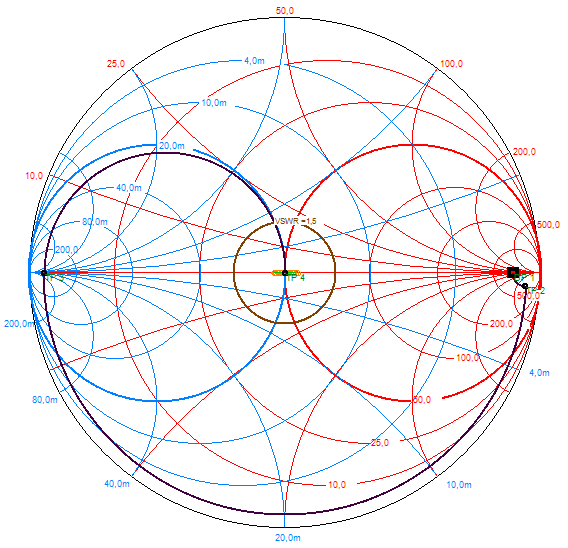
\includegraphics[scale=0.43]{imagenes/smith_4_espacio_libre.png}
%	\label{fig.smith_4}
%\end{figure}


Por otra parte, a partir de la herramienta \textit{Sweep Over Frequency} de \textit{Smith}, se dedujo que no se cumple el criterio de adaptación $|\rho_L|< 0,2$.

\subsection{Stub}

La adaptación mediante \texttt{stub} consiste en anexar un trozo de la misma línea conectada en paralelo. Normalmente, para evitar interferencias se suele cortocircuitar el extremo de la carga. La longitud del stub se denota $l_s$ y la distancia a la carga $l_o$


%%%% FIGURA PARA STUB ESPACIO LIBRE
%\begin{figure}[H]
%	\centering
%	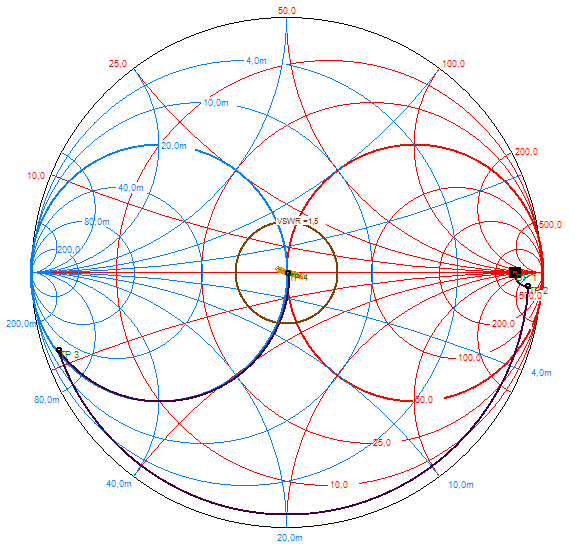
\includegraphics[scale=0.43]{imagenes/smith_stub_espacio_libre.png}
%	\label{fig.smith_stub}
%\end{figure}


Mediante el \textit{Smith} se obtuvieron los parámetros

\begin{equation}
	\centering
	l_o = \frac{\lambda}{2 \cdot \pi} atan(\sqrt{Z_l / Z_o})
\end{equation}


